\section{404 pages}

The site has not developed a specific page to handle the case in which the 
user requests a specific page that does not exist. You can find two 
different 404 pages: figure \ref{fig:404-academy} illustrates the result 
if a non-existent \textit{Academy} article is searched and figure 
\ref{fig:404-support} illustrates the result if non-existent content of the 
page \textit{Supporto} is searched. These pages are very raw and do not 
provide useful information to the user. The use of the error code 404 can 
be omitted, as it represents a technicality that is not helpful to the 
user. The link to return to the homepage in figure \ref{fig:404-support} 
also represents a reference to be able to return to a familiar point for 
the user, however it also represents a disadvantage: if the user has reached 
this non-existent page via the \textit{deep linking}, making the user go 
back would mean leaving the site. In the figure \ref{fig:404-academy} it 
is possible to see that the 404 page is not managed well: apart from the 
ironic phrase, all the texts of the menus, buttons and footer are not 
loaded. This can cause severe disorientation for the user. Among other 
things, being the section of learning articles, therefore frequented 
above all by novice users, it does not contribute to maintaining a good 
level of quality.

\begin{figure}[H]
  \centering
  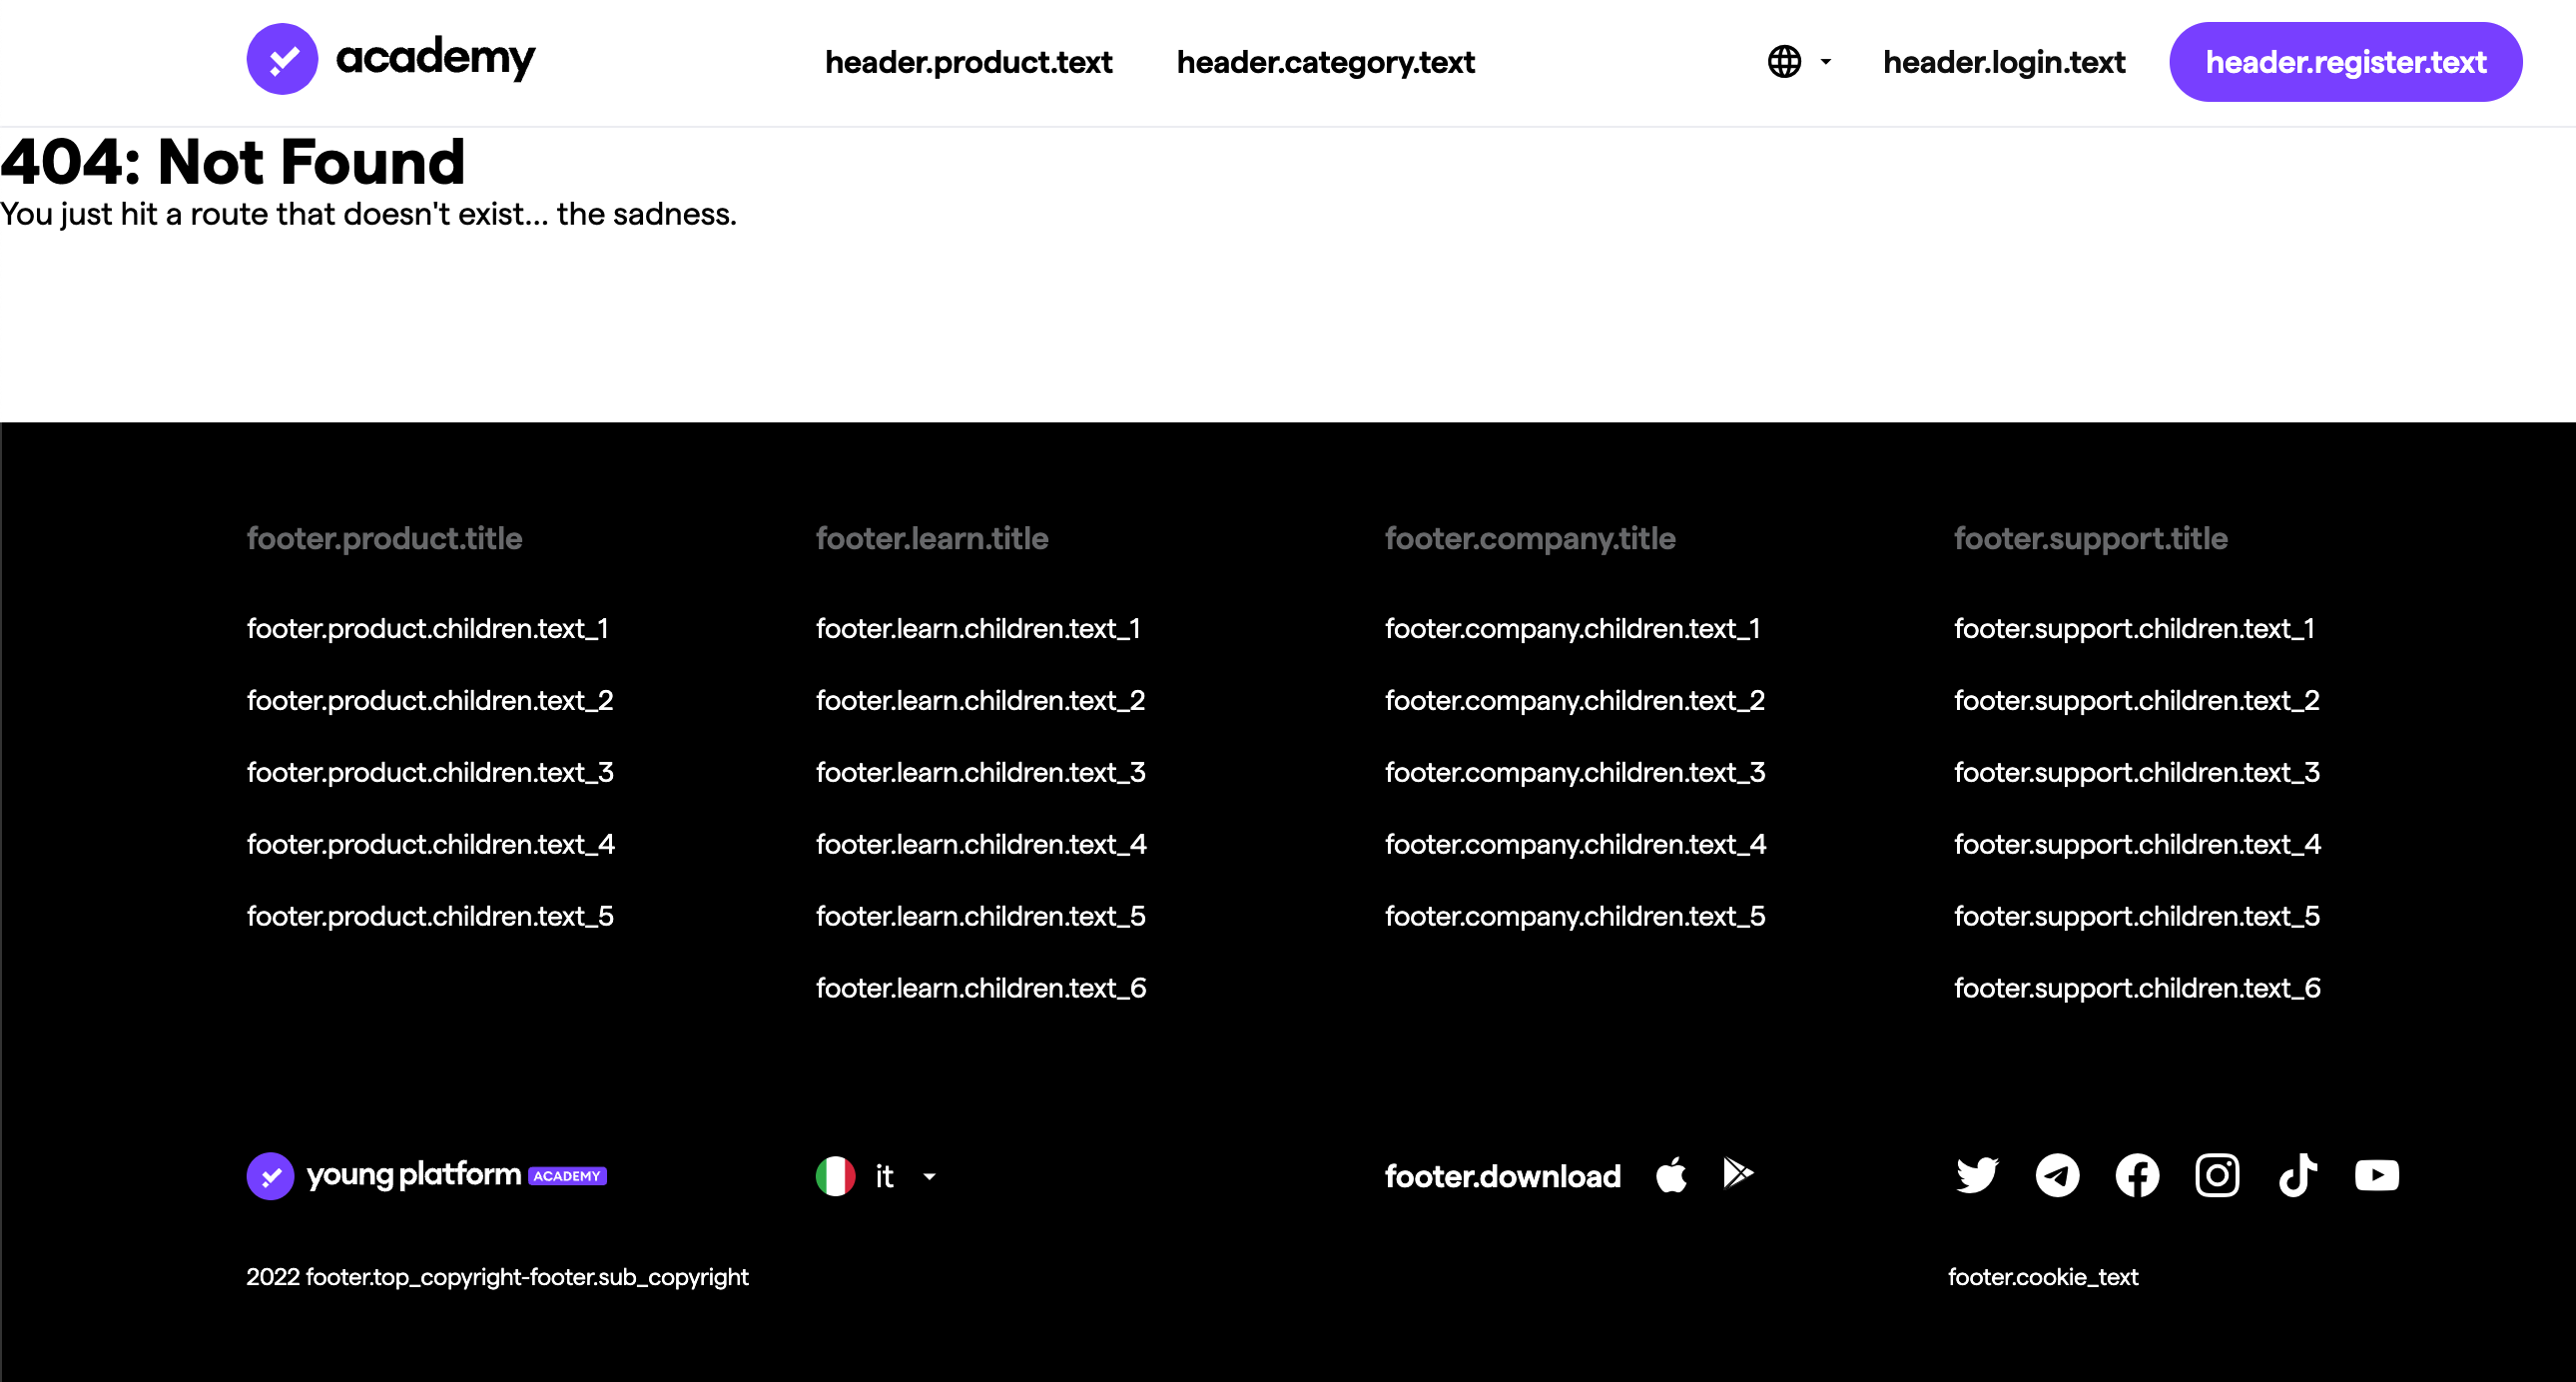
\includegraphics[width=0.80\textwidth]{res/images/404-academy.png}
  \caption{Page 404 which occurs if an article from the \textit{Academy} 
  page is not found.}
  \label{fig:404-academy}
\end{figure}

\begin{figure}[H]
  \centering
  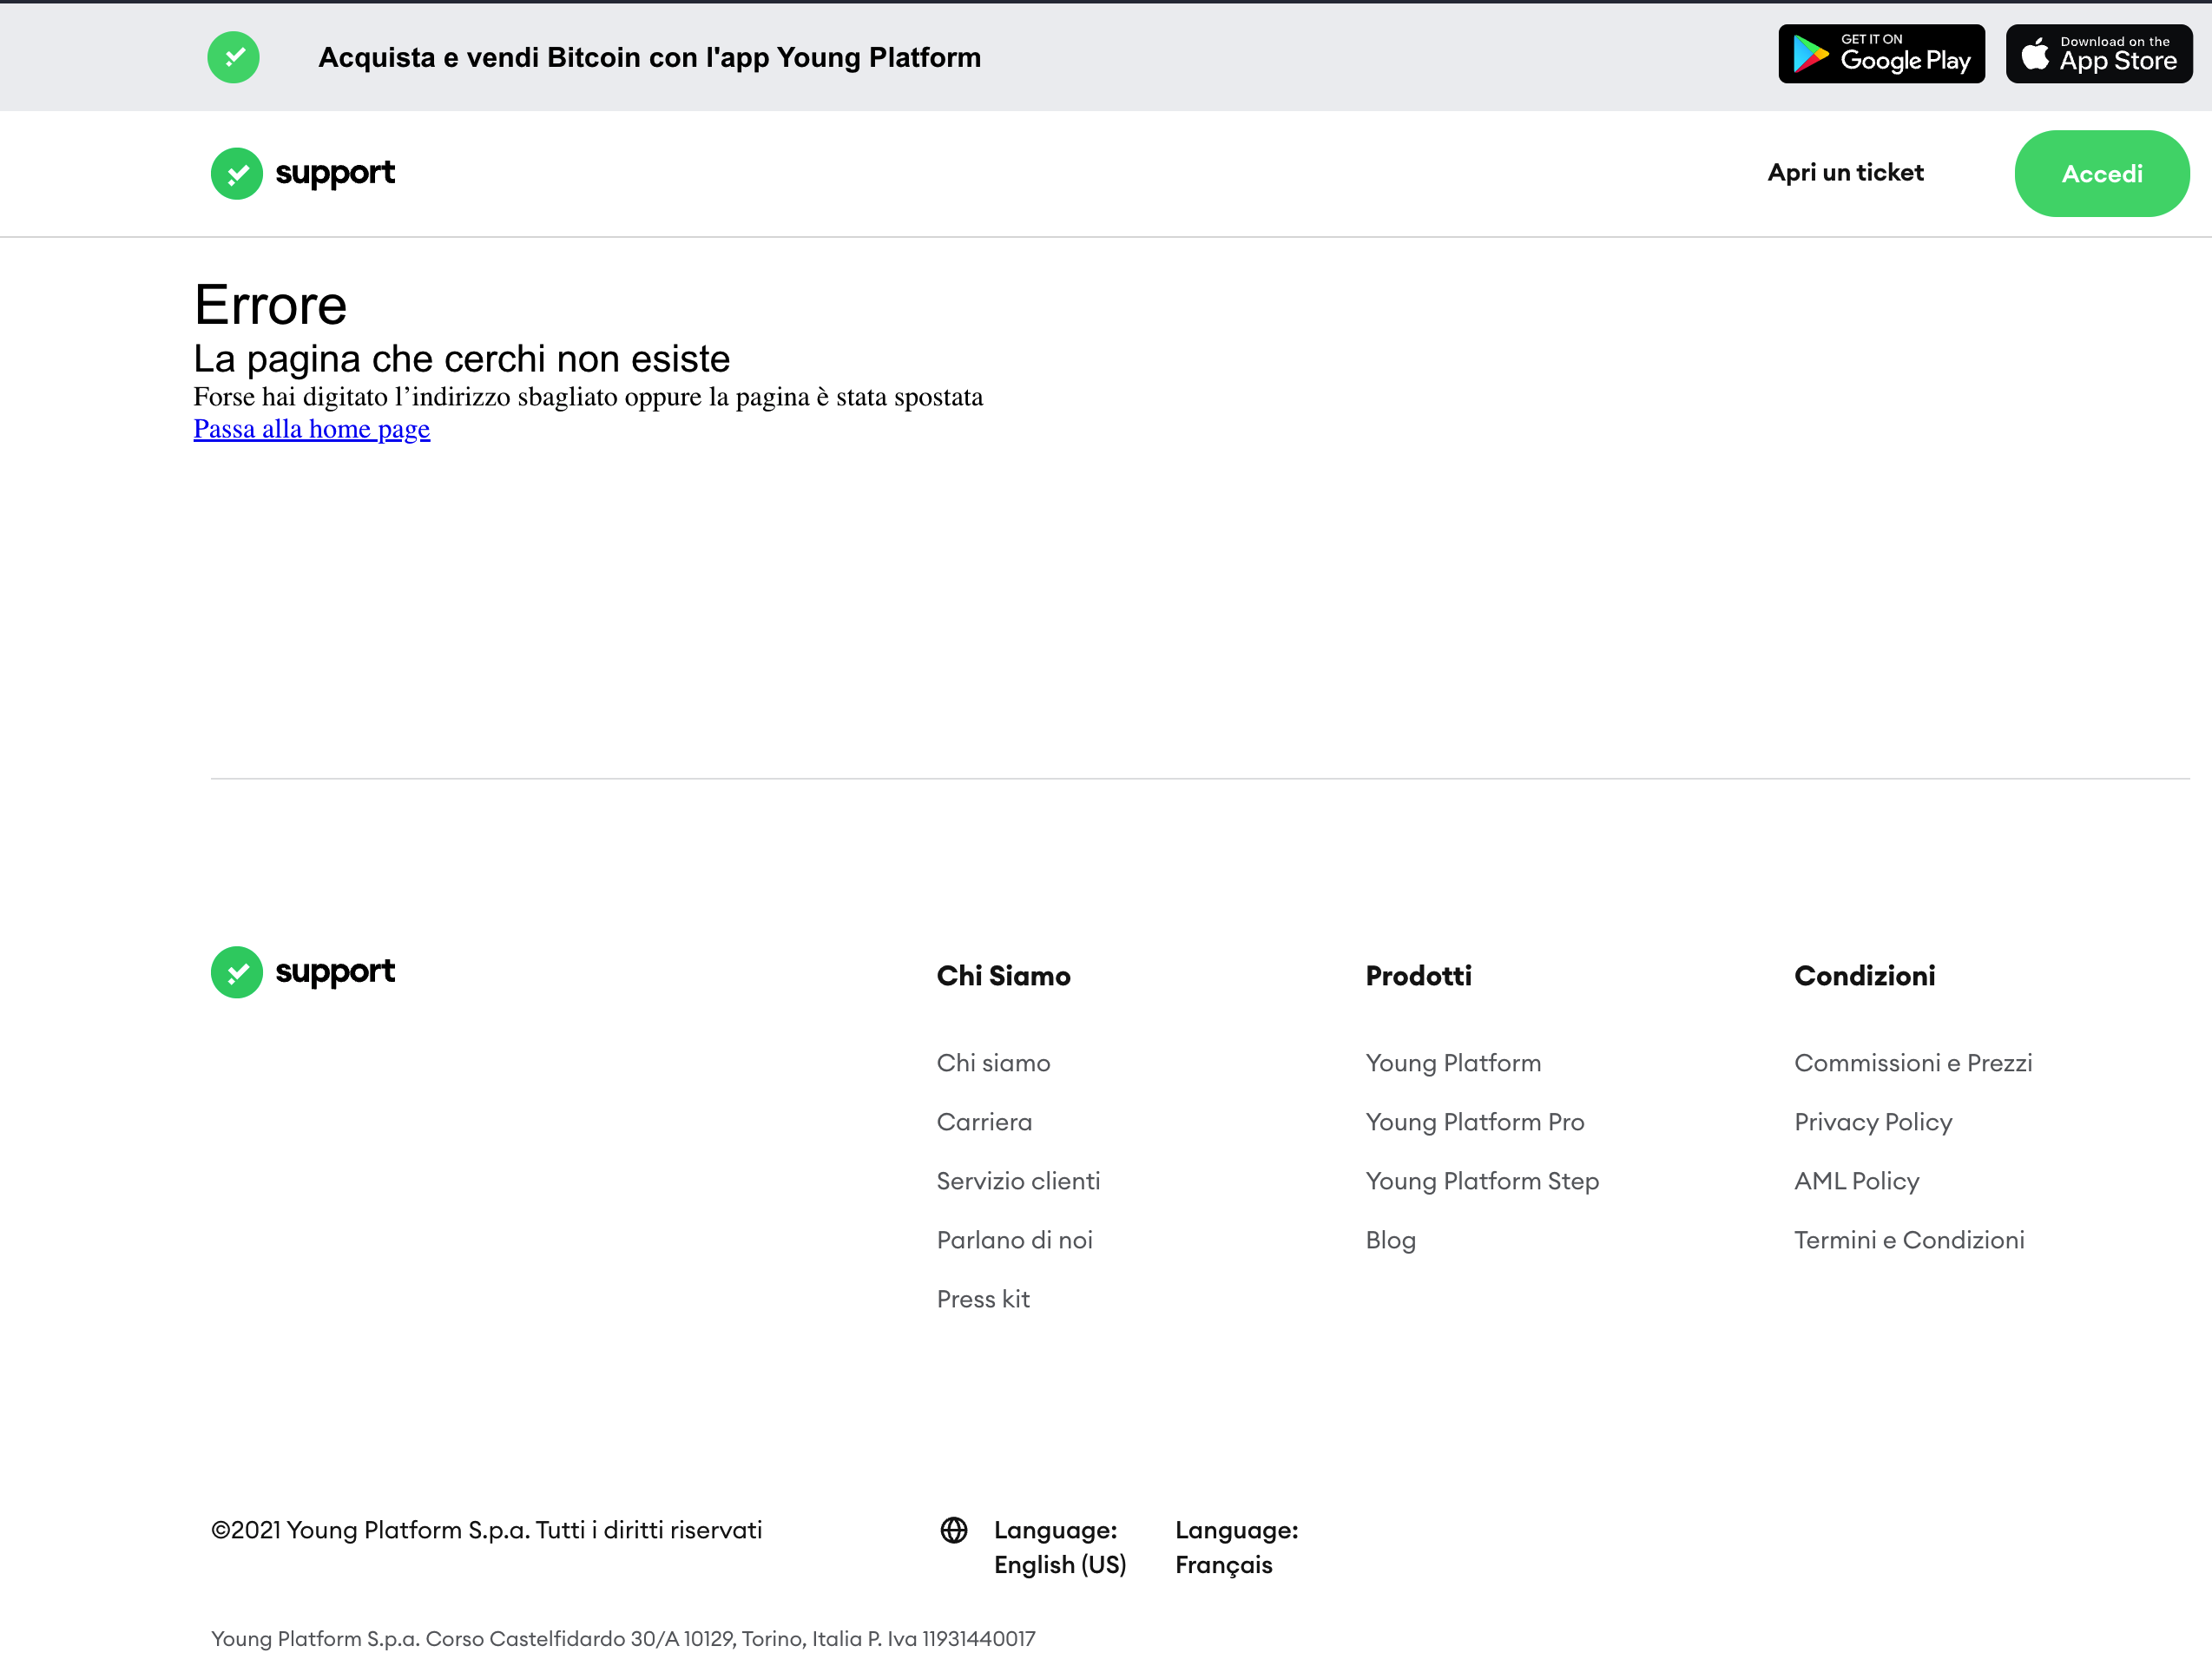
\includegraphics[width=0.80\textwidth]{res/images/404-support.png}
  \caption{Page 404 which appears if you search for content not present 
  in the page \textit{Supporto}.}
  \label{fig:404-support}
\end{figure}